\documentclass{article}

\usepackage[english]{babel}
\usepackage[letterpaper,top=2cm,bottom=2cm,left=3cm,right=3cm,marginparwidth=1.75cm]{geometry}
\usepackage{amsmath}
\usepackage{amssymb}
\usepackage{amsthm}
\usepackage{comment}
\usepackage{enumitem}
\usepackage{graphicx}
\usepackage[colorlinks=true, allcolors=blue]{hyperref}
\usepackage[skip=20pt, indent=0pt]{parskip}
\usepackage{tikz}
    \usetikzlibrary{calc}

% \linespread{1.5}
\newtheorem*{lemma}{Lemma}

\title{Math 134 A Homework 1}
\author{Alexandre Lipson}

\begin{document}
\maketitle

\section*{1.2}

\subsection*{70}
Show that the sum of two rational numbers is rational.

Assume that if $a,b \in \mathbb{Z}$, then $a + b \in \mathbb{Z}$ and $ab \in \mathbb{Z}$.

Assume $\mathbb{Q} = \frac{p}{q} : p,q \in \mathbb{Z}, q \neq 0$.

Let $x = \frac{a}{b}$ and $y = \frac{c}{d}$ where $a,b,c,d \in \mathbb{Z}$ and $b,d \neq 0$ so that $x, y \in \mathbb{Q}$.

Then $\frac{a}{b} + \frac{c}{d} = \frac{ad + bc}{bd}$.

Since $a,b,c,d \in \mathbb{Z}$, then $bd \in \mathbb{Z}$ by the first assumption.
Since $b,q \neq 0$, then $bd \neq 0$.

Since $ad,bc \in \mathbb{Z}$, it follows that $ad + bc \in \mathbb{Z}$ by the first assumption.

Since both $ad + bc \in \mathbb{Z}$ and $0 \neq bd \in \mathbb{Z}$, then $\frac{ad + bc}{bd} \in \mathbb{Z}$.

Therefore the sum of two rational numbers, $\frac{a}{b} + \frac{c}{d} = \frac{ad + bc}{bd}$, is rational.


\subsection*{71}
Show that the sum of a rational and an irrational is irrational.

For a contradiction, assume $x + y \in \mathbb{Q} : x \in \mathbb{Q}, y \in \mathbb{R} \setminus \mathbb{Q}$.

Since $\mathbb{Q} = \left\{ \frac{p}{q} : p,q \in \mathbb{Z}, q \neq 0 \right\}$,

Then $x = \frac{a}{b}$ where $a,b \in \mathbb{Z}, b \neq 0$.

So, $x + y = \frac{a}{b} + \frac{y}{1}$ where $y = \frac{y}{1}$.

Then, $x + y = \frac{a + by}{b}$.

We can assume that both the sum and product of an integer with an irrational will not produce an integer.

Therefore, $a + by \notin \mathbb{Z}$.

Since the numerator is not an integer, the definition of a rational does not hold. 

Therefore, $x + y \notin \mathbb{Q}$ where $x \in \mathbb{Q}, y \in \mathbb{R} \setminus \mathbb{Q}$.



\subsection*{74}
Show by example that the sum of two irrational numbers can be either be rational or irrational. 
Do the same for the product of two irrational numbers.

Assume $e \in \mathbb{R} \setminus \mathbb{Q}$.

Assume that a real number can either be rational or irrational.

Assume that the product of an integer and an irrational is not an integer.

Assume that the sum of a rational with an irrational is irrational.\footnote{see 1.2 71.}

\vspace{12pt}

Let $e + e = 2e = \frac{2e}{1}$.

Since $2e \notin \mathbb{Z}$ by assumption three, then $\frac{2e}{1} \notin \mathbb{Q}$.

So, $2e \in \mathbb{R} \setminus \mathbb{Q}$ by assumption two.

Therefore, the sum of two irrationals can produce an irrational.

\vspace{12pt}

Let $a = x + e$ and $b = x - e$ where $x \in \mathbb{Q}$.

So $a, b \in \mathbb{R} \setminus \mathbb{Q}$.

Then, $a + b = (x + e) + (x - e) = x$

Therefore, the sum of two irrationals can produce a rational.

\vspace{12pt}

Let $e(e) = e^2$.

Since $e^2 \in \mathbb{R} \setminus \mathbb{Q}$, then the product of two irrationals can be irrational.

\vspace{12pt}

Let $a = e$ and $b = \frac{1}{e}$.

So, $a, b \in \mathbb{R} \setminus \mathbb{Q}$

Then, $ab = \frac{e}{e} = 1$.

Since $1 \in \mathbb{Q}$, the product of two irrationals can produce a rational.



\section*{1.3}

\subsection*{53}
Show that $\bigl| |a|-|b| \bigr| \leq |a-b| $ for all real numbers $a$ and $b$. (By calculating $\bigl||a|-|b|\bigr|^2$)

Assume $|a| = \sqrt{a^2}$ and therefore $|a|^2 = a^2$.

For any $x \in \mathbb{R}$, if $x \geq 0$, then $x = |x|$. Else, $x < 0 \leq |x|$.

Therefore $x \leq |x|$.

Then, with $x = ab$, $ab \leq |ab|$.

Then, 
\begin{align*}
    |ab| &= \sqrt{{(ab)}^2} \text{ by the assumption.} \\
         &= \sqrt{{a}^2 {b}^2} \\
         &= \sqrt{a^2} \sqrt{b^2} \\
         &= |a||b|
\end{align*}

So, $ab \leq |ab| = |a||b|$.

Then,
\begin{align*}
    -2ab &\geq -2|a||b| \\
    a^2 - 2ab + b^2 &\geq a^2 - 2|a||b| + b^2 \\
    a^2 - 2ab + b^2 &\geq |a|^2 - 2|a||b| + |b|^2 \text{ by the assumption.} \\
    {(a - b)}^2 &\geq {(|a| - |b|)}^2 \\
    {|a - b|}^2 &\geq {\bigl| |a|-|b| \bigr|}^2 \text{ again, by the assumption.} \\
    |a - b| &\geq \bigl| |a|-|b| \bigr|.
\end{align*}

So, the statement holds.


\subsection*{58}
Given that $0 \leq a \leq b$, show that \[a \leq \sqrt{ab} \leq \frac{a+b}{2} \leq b.\] 
The number $\sqrt{ab}$ is called the \textit{geometric mean} of $a$ and $b$.

Assume $x = \sqrt{x^2}$.

For $x \geq 0 \in \mathbb{R}$, if $x \geq 4$, then $\frac{x}{2} \geq \sqrt{x}$ else $\frac{x}{2} < \sqrt{x}$.

Since $a \leq b$, then
\begin{align*}
    a^2 &\leq ab \\
    \sqrt{a^2} &\leq \sqrt{ab} \\
    a &\leq \sqrt{ab} \text{ by the assumption.} \\
\end{align*}

Since $b \geq a$, then
\begin{align*}
    0 &\leq b-a \\
    0 &\leq {(b-a)}^2 \\
    0 &\leq a^2 - 2ab + b^2 \\
    4ab &\leq a^2 + 2ab + b^2 \\
    4ab &\leq {(a+b)}^2 \\
    \sqrt{4ab} &\leq a+b \\
    \sqrt{ab} &\leq \frac{a+b}{2} \\
\end{align*} 

Therefore, $\sqrt{ab} \leq \frac{a+b}{2}$ holds.


Since $a \leq b$, then
\begin{align*}
    \frac{a}{2} &\leq \frac{b}{2} \\
    \frac{a}{2} + \frac{b}{2} &\leq \frac{b}{2} + \frac{b}{2} \\
    \frac{a + b}{2} &\leq b \\
\end{align*}

Therefore, $\frac{a + b}{2} \leq b$ holds.

Since all of the inequalities: $a \leq \sqrt{ab}$, $\sqrt{ab} \leq \frac{a+b}{2}$, and $\frac{a+b}{2} \leq b$ are true separately,
$a \leq \sqrt{ab} \leq \frac{a+b}{2} \leq b$ is also true.


\section*{1.4}

\subsection*{52}

The \textit{perpendicular bisector} of the line segment $\overline{PQ}$ is the line which is perpendicular to $\overline{PQ}$ 
and passes through the midpoint of $\overline{PQ}$. 

Find an equation for the perpendicular bisector of the line segment that joins the two points. 
\\ $P = (-1,3)$ and $Q = (3,-4)$

% not written in a very proof-like manner
First, we find the midpoint of segment $\overline{PQ}$.
\[M = \left( \frac{(-1)+3}{2}, \frac{3+(-4)}{2}\right) = \left( 1, \frac{-1}{2} \right)\]

Next, find the slope of $\overline{PQ}$.
\[m = \frac{3-(-4)}{(-1)-3} = -7/4\]

The perpendicular to this slope is given by the negative reciprocal $\frac{-1}{m}$.

So, the slope of the perpendicular bisector is $\frac{4}{7}$.

Find the equation of the perpendicular bisector using the point-slope form $y-y_1 = m(x-x_1)$ 
where $(x_1,y_1)$ is a point on the line and $m$ is the slope of the line.

So,
\begin{align*}
   y - \left( -\frac{1}{2} \right) &= \frac{4}{7} (x - 1) \\
   y &= \frac{4}{7}x - \frac{4}{7} - \frac{1}{2} \\
   y &= \frac{4}{7}x - \frac{11}{14} \\
\end{align*}

So, the equation of the perpendicular bisector of $\overline{PQ}$ is
\[y = \frac{4}{7}x - \frac{11}{14}.\]


\subsection*{62}

Show that the medians of a triangle intersect in a single point (called the \textit{centroid} of the triangle). 
Introduce a coordinate system such that one vertex is at the origin and one side is on the positive x-axis.

\begin{figure*}[ht] %h: place figure about here
\centering
\begin{tikzpicture}
    \draw[->] (-0.75,0) -- (4,0) node[below] {$x$};
    \draw[->] (0,-0.75) -- (0,2.5) node[left] {$y$};

    \coordinate (origin) at (0,0);
    \coordinate (c) at (2.75,0);
    \coordinate (a_b) at (2,1.5);

    \draw (origin) -- (c) -- (a_b) --cycle;

    \node[below] at (c) {($c$, 0)};
    \node[above right] at (a_b) {($a$, $b$)};

    \fill (c) circle[radius=2pt];
    \fill (a_b) circle[radius=2pt];
\end{tikzpicture}
\end{figure*}

We will set up a system of three linear equations each representing one of the medians of the triangle.

Let the slope of a line $m$ be defined as $\frac{y_1-y_0}{x_1-x_0}$ where $(x_0,y_0)$ and $(x_1,y_1)$ are two given points.

Let the equation of a line $f$ given a slope $m$ and point $(x_0,y_0)$ be the point slope form $y-y_0 = m(x-x_0)$.

Let line $f$ be defined by the origin $(0,0)$ and the midpoint of edge opposing the origin $\left( \frac{a+c}{2}, \frac{b}{2} \right)$.

$m_f = \frac{b}{a+c} x$ by the first definition.

So, $f(x) = \frac{b}{a+c} x$ by the second definition.

Let line $g$ be defined by the top point $(a,b)$ and the midpoint of the base $\left( \frac{c}{2}, 0 \right)$.

$m_g = \frac{b-0}{a-\frac{c}{2}} = \frac{2b}{2a-c}$ by the first definition.

So, 
\begin{align*}
    g-b &= \frac{2b}{2a-c} (x-a) \text{ by the second definition.}\\
    &= \frac{2b(x-a)+b(2a-c)}{2a-c} \\
    &= \frac{b(2x-2a+2a-c)}{2a-c} \\
    g(x) &= \frac{b(2x-c)}{2a-c} \\
\end{align*}

Let line $h$ be defined by the right point $(c,0)$ and the midpoint of the upper edge $\left( \frac{a}{2}, \frac{b}{2} \right)$.

$m_h = \frac{0-\frac{b}{2}}{c-\frac{a}{2}} = \frac{b}{a-2c}$ by the first definition.

So, $h(x) = \frac{b}{a-2c} (x-c)$ by the second definition.

The medians are visualized in the following \href{https://www.desmos.com/calculator/fowljkwimc}{figure}.

\begin{figure*}[ht] %h: place figure about here
\centering
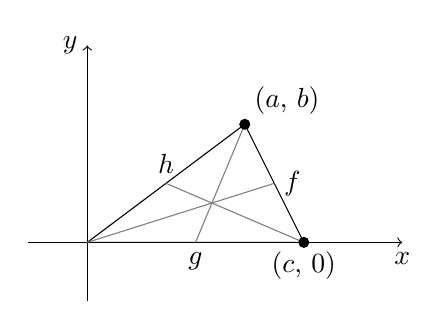
\begin{tikzpicture}
    \draw[->] (-0.75,0) -- (4,0) node[below] {$x$};
    \draw[->] (0,-0.75) -- (0,2.5) node[left] {$y$};

    \coordinate (origin) at (0,0);
    \coordinate (c) at (2.75,0);
    \coordinate (a_b) at (2,1.5);

    \coordinate (mid_base) at (1.375,0);
    \coordinate (mid_opp) at (2.375,0.75);
    \coordinate (mid_top) at (1,0.75);

    \draw (origin) -- (c) -- (a_b) --cycle;

    \draw[gray] (origin) -- (mid_opp);
    \draw[gray] (a_b) -- (mid_base);
    \draw[gray] (c) -- (mid_top);

    \node[right] at (mid_opp) {$f$};
    \node[below] at (mid_base) {$g$};
    \node[above] at (mid_top) {$h$};

    \node[below] at (c) {($c$, 0)};
    \node[above right] at (a_b) {($a$, $b$)};

    \fill (c) circle[radius=2pt];
    \fill (a_b) circle[radius=2pt];
\end{tikzpicture}
\end{figure*}

Then, we show that the lines $f$ and $g$ are equal at some $x$.
\begin{align*}
    \frac{b}{a+c} x &= \frac{b(2x-c)}{2a-c} \\
    \frac{b}{a+c} x &= \frac{2bx}{2a-c} - \frac{bc}{2a-c} \\
    b(2a-c) x &= 2bx(a+c) - bc(a+c) \\
    (b(2a-c) - 2b(a+c)) x &= -bc(a+c) \\
    (2ab - bc - 2bc - 2ab) x &= -bc(a+c) \\
    -3bcx &= -bc(a+c) \\
    x &= \frac{a+c}{3} \\
\end{align*}

So, the lines intersect at $x$.

Let $P$ be the intersection point of $f$ and $g$ given by $f$ evaluated at $x = \frac{c-a}{3}$.
\begin{align*}
    f(x) &= \frac{b}{a+c} x \\
    f\left(\frac{a+c}{3}\right) &= \left(\frac{b}{a+c}\right)\left(\frac{a+c}{3}\right) \\
    &= \frac{b}{3}\\
\end{align*}

So, \[P = \left(\frac{a+c}{3}, \quad \frac{b}{3}\right)\]

Then, we will show that $P$ is on the third line $h$.

Since $h(x) = \frac{b}{a-2c} (x-c)$, then
\begin{align*}
    h\left(\frac{a+c}{2}\right) &= \frac{b}{a-2c} \left(\frac{a+c}{3}-c\right) \\
    &= \frac{b}{a-2c} \left(\frac{a-2c}{3}\right) \\
    &= \frac{b}{3} \\
\end{align*}

So, $h\left( \frac{a+c}{2} \right) = \frac{b}{3}$ which satisfies $P$.

Since the intersection point $P$ of lines $f$ and $g$ also lies on $h$, then all three lines intersect.

Therefore, the medians of a triangle intersect.

\section*{1.6}

\subsection*{80}

Show that Dirichlet's function $ f(x) = \begin{cases} 
    0 & \text{$x$ rational} \\
    0 & \text{$x$ irrational}
\end{cases}$ is periodic but has no period.
% second part is proof by contradiction

Let a function be $f$ periodic such that $f(a) = f(a + p)$, $p \neq 0$, and $a, a+p$ are both in the domain of $f$. 
The smallest number $p$ to satisfy this property for $f$ is the period.

Assume that the sum of two rationals is rational.\footnote{see 1.2 70.}

Assume that the sum of a rational and an irrational is irrational.\footnote{see 1.2 71.}

%Assume that the product of two rationals is rational.

If $a \in \mathbb{R}$, then there are two cases to demonstrate, $a$ is either rational or irrational.

Let $k \in \mathbb{Q}$.

If $a \in \mathbb{Q}$, then $f(a) = 1$.
Since $a+k \in \mathbb{Q}$ by the first assumption, then $f(a+k) = 1$.

If $a \in \mathbb{R} \setminus \mathbb{Q}$, then $f(a) = 0$.
Since $a+k \in \mathbb{R} \setminus \mathbb{Q}$ by the second assumption, then $f(a+k) = 0$.

Therefore, $f$ is periodic by the definition as all cases are covered.

%% proof by contradiction & induction?
Then, for a contradiction, assume that $f$ has a smallest period $T>0 \in \mathbb{R}$.

So, $f(a) = f(a+T)$.

\begin{lemma}
    For any real number $a$, there exists a rational number $b$ such that $b<a$. 
    \[\forall x \in \mathbb{R}. \ \exists b \in \mathbb{Q} : b<a.\]
\end{lemma}

\begin{proof}
    We will look at two cases: $a$ is either rational or irrational.

    First, if $a \in \mathbb{Q}$, then $a > \frac{a}{2} \in \mathbb{Q}$.
    
    Second, if $a \in \mathbb{R} \setminus \mathbb{Q}$, then a will not have a repeating decimal expansion.

    Since, $a$ does not have a repeating decimal expansion, we can create a smaller number $b$ with a repeating expansion
    by only including a some digits of the decimal expansion of $a$ while letting the remaining digits be repeating zeros.
    
    Then $a-b$ will produce the digits not included in the rational $b$. 

    So, $a-b>0$.

    Since $a-b>0$, then $a>b$.

    Therefore, a rational $b$ can always be found less than a given real number $a$.\qedhere
\end{proof}

There exists $0 < T' < T : T' \in \mathbb{Q}$ by the lemma. 

Since $T' \in \mathbb{Q}$, then $f(a) = f(a+T')$ by above.

So, we have found a smaller period and therefore the statement does not hold.

Therefore, there is no smallest period $T$ for $f$ and thus $f$ has no period.

\section*{1.7}

\subsection*{59}

Show that every function defined for all real numbers can be written as the sum of an even function and an odd function.

Let even functions be defined such that, for an even function $E$, $E(-x) = E(x)$.
\begin{align*}
    2E(x) &= E(-x) + E(x) \\
    E(x) &= \frac{E(-x)+E(x)}{2}
\end{align*}

Likewise, let the odd function $O$ be defined by, $O(-x) = -O(x)$.
\begin{align*}
    2O(x) &= O(-x) - O(x) \\
    O(x) &= \frac{E(-x)-E(x)}{2}
\end{align*}

Let $f(x) : x \in \mathbb{R}$ be defined as the sum of $E$ and $O$. 
\[f(x) = E(x) + O(x)\]

So, $f(-x) = E(-x) + O(-x)$.

Then, $f(-x) = E(x) - O(x)$ by the definition.

Then, $f(x) + f(-x) = 2E(x)$. 
So, $f(-x) + f(x) = 2E(-x)$, which is also $2E(x)$ by the definition.
Therefore, $E(x) = \frac{f(x) + f(-x)}{2}$.

Which matches the definition of even functions.

Then, $f(x) - f(-x) = 2O(x)$.
So, $O(x) = \frac{f(x) - f(-x)}{2}$.

Which matches the definition of odd functions.

Therefore any function $f$ can be defined as the sum of an even and odd function.

\section*{1.8}

\subsection*{6}

Show that the following statement holds for all positive integers $n$,
\[1^3+2^3+3^3+\cdots+n^3 = {(1+2+3+\cdots+n)}^2.\] 
%Use $2n \leq 2^n$.

First we rewrite the statement, \[ \sum\limits_{i=1}^{n} i^3 = {\left( \sum\limits_{i=1}^{n} i \right)}^2 \]

% Lemma 1
\begin{lemma}
    $\sum\limits_{i=1}^{n} i = \frac{n(n+1)}{2} : n \in \mathbb{Z}^{+}$
\end{lemma}

\begin{proof}
    We will prove by induction that $\sum\limits_{i=1}^{n} i = \frac{n(n+1)}{2}$ for all positive integers $n$.

    Let $S=\mathbb{Z}^{+}$
    
    When $n=1 \in S$, \[1=\frac{1(1+1)}{2}.\] % induction step
    
    So, the statement holds for the base case $n=1$.
    
    Now, for $k \in S$, we assume that the formula holds for $n=k$. % induction hypothesis
    
    Then, sum the first $k+1$ integers where $n=k+1 \in S$.
    
    \begin{align*}
        \sum\limits_{i=1}^{k} i + (k+1) &= \frac{k(k+1)}{2} + (k+1) \text{ by the induction hypothesis.} \\ % point out where induction hypothesis is used
        \sum\limits_{i=1}^{k+1} i &= \frac{k(k+1)+2(k+1)}{2} \\
        &= \frac{(k+1)(k+2)}{2} \\
        &= \frac{(k+1)[(k+1)+1]}{2} \\
    \end{align*}
    
    
    Which is the formula with $n=k+1$. 
    % conclusion
    Therefore, by induction, the formula holds for all $n \in S$.\qedhere       
\end{proof}

\begin{lemma}
    $\sum\limits_{i=1}^{n} i^3 = {\left( \frac{n(n+1)}{2} \right)}^2 : n \in \mathbb{Z}^{+}$.
\end{lemma}

\begin{proof}        
    We will show that \[\sum\limits_{i=1}^{n} i^3 = {\left( \frac{n(n+1)}{2} \right)}^2\] 
    by induction on $n$ for all positive integers $S = \mathbb{Z}^{+}$.

    For the base case, when $n=1 \in S$, \[1^3 = {\left( \frac{1(1+1)}{2} \right)}^2 = 1^2 = 1.\]

    So, the formula holds for the step $n=1$.

    Assume that the formula holds for $n=k \in S$.

    Then, for $n=k+1 \in S$, by the induction hypothesis,

    \begin{align*}
        \sum\limits_{i=1}^{k} i^3 + {(k+1)}^3 &= {\left( \frac{k(k+1)}{2} \right)}^2 + {(k+1)}^3 \\
        \sum\limits_{i=1}^{k+1} i^3 &= {\left( \frac{k(k+1)}{2} \right)}^2 + {(k+1)}^3 \\
        &= \frac{k^2 {(k+1)}^2}{4} + \frac{4(k+1){(k+1)}^2}{4} \\
        &= \frac{(k^2+4k+4){(k+1)}^2}{4} \\
        &= \frac{{(k+2)}^2 {(k+1)}^2}{2^2} \\
        &= {\left( \frac{(k+1)(k+2)}{2} \right)}^2 \\
        &= {\left( \frac{(k+1)[(k+1)+1]}{2} \right)}^2 \\
    \end{align*}

    Which is the same as the formula where $n=k+1$.

    Therefore, by induction, the statement holds for all $n \in S$.\qedhere

\end{proof}

Using the two lemmas, we can again rewrite the original statement, 
\[{\left( \frac{n(n+1)}{2} \right)}^2 = {\left( \frac{n(n+1)}{2} \right)}^2\]

So, we can see that the statement holds.

%We can also prove via induction with an additional ${(k+1)}^3$ or $k^3$--if we set up the induction hypothesis using $n=k-1$.

\subsection*{18}

Show that, given a unit length, for each $n$ in the set of positive integers $S$, 
a line segment of length $\sqrt{n}$ can be constructed by straight edge and compass.

Assume that, with a straight edge and compass, a perpendicular line can always be constructed to any line segment.

Pythagorean theorem: 
Assume that for a right triangle with side lengths $a$ and $b$, the hypotenuse will be given by $\sqrt{a^2 + b^2}$.

We will prove by induction on $n \in S = \mathbb{Z}^{+}$ that a segment of length $\sqrt{n}$ can be constructed by a chain of triangles 
where the subsequent triangle is constructed by using hypotenuse of the previous as the base in addition to a height of the unit length.

\begin{figure*}[ht]
\centering
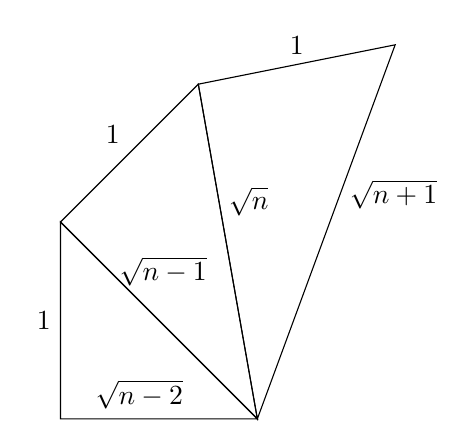
\begin{tikzpicture}
    \coordinate (A) at (0,0);
    \coordinate (B) at (2.5,0);
    \coordinate (C) at (0,2.5);
    \coordinate (D) at (1.75,4.25);
    \coordinate (E) at (4.25,4.75);

    \draw (A) -- (B) -- (C) -- cycle;
    \draw (B) -- (C) -- (D) -- cycle;
    \draw (B) -- (D) -- (E) -- cycle;
  
    \node[left] at ($(A)!0.5!(C)$) {$1$};
    \node[above left] at ($(C)!0.5!(D)$) {$1$};
    \node[above] at ($(D)!0.5!(E)$) {$1$};

    \node[above] at ($(A)!0.4!(B)$) {$\sqrt{n-2}$};
    \node[right] at ($(B)!0.75!(C)$) {$\sqrt{n-1}$};
    \node[right] at ($(B)!0.65!(D)$) {$\sqrt{n}$};
    \node[right] at ($(B)!0.6!(E)$) {$\sqrt{n+1}$};
  \end{tikzpicture}
\end{figure*}

Let the unit length be $1$.

Since, for $n=1$, we immediately get the line segment of length $\sqrt{n}$ from the fact that $1 = \sqrt{1}$. 

So, the induction base case will start at $n=2$.

Then, for $n=2$, create an isosceles right triangle with a base and height of the unit length.

\begin{figure*}[ht]
\centering
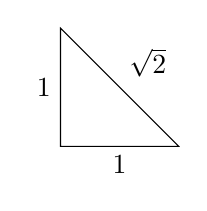
\begin{tikzpicture}
    \coordinate (A) at (0,0);
    \coordinate (B) at (1.5,0);
    \coordinate (C) at (0,1.5);

    \draw (A) -- (B) -- (C) -- cycle;
  
    \node[below] at ($(A)!0.5!(B)$) {$1$}; % Base
    \node[left] at ($(A)!0.5!(C)$) {$1$};  % Height
    \node[above right] at ($(B)!0.5!(C)$) {$\sqrt{2}$}; % Hypotenuse
  \end{tikzpicture}
\end{figure*}

So, \[\sqrt{1^2 + 1^2} = \sqrt{2}.\]

We will assume that for $n=k \in S$, we can construct a line segment of length $\sqrt{k}$ by the induction hypothesis.

Then, given a segment of $\sqrt{k}$, we can find a segment $\sqrt{k+1}$ by the Pythagorean theorem.
\\ Construct a perpendicular line segment of the unit length on one side of $\sqrt{k}$.
\\ Connect the distant endpoints of the unit segment and the $\sqrt{k}$ segment.
\\ This will form a right triangle with base lengths of $1$ and $\sqrt{k}$.

So,
\begin{align*}
    \sqrt{k+1} &= \sqrt{{\left( \sqrt{k} \right)}^2 + 1^2} \text{ by the Pythagorean theorem.} \\
    &= \sqrt{k+1} \\
\end{align*}

\begin{figure*}[ht]
\centering
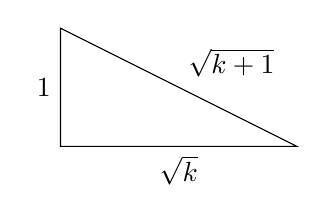
\begin{tikzpicture}
    \coordinate (A) at (0,0);
    \coordinate (B) at (3,0);
    \coordinate (C) at (0,1.5);

    \draw (A) -- (B) -- (C) -- cycle;
  
    \node[below] at ($(A)!0.5!(B)$) {$\sqrt{k}$}; % Base
    \node[left] at ($(A)!0.5!(C)$) {$1$};  % Height
    \node[above right] at ($(B)!0.5!(C)$) {$\sqrt{k+1}$}; % Hypotenuse
  \end{tikzpicture}
\end{figure*}

Therefore, since we can construct a segment with length $\sqrt{k+1}$ from a segment of $\sqrt{k}$, the statement is true.

\end{document}